%==============================================================================
% Counterfactual Shadow Control -- IEEE Internet of Things Journal
%
% TARGET: 6.0 published pages INCLUDING references. Hard ceiling 8.
% Figures: exactly 4.  Tables: exactly 3.
%
% RULE: every number in Section V is produced by analysis/ from
% results_long.csv and pulled in with \input. A number typed by hand in
% Section V is a bug. Section V, the abstract, and Figs. 3-4 stay as
% placeholders until BACKLOG.md phase 16 is complete.
%==============================================================================
\documentclass[journal]{IEEEtran}

\usepackage{amsmath,amssymb}
\usepackage{booktabs}
\usepackage{graphicx}
\usepackage{tikz}
\usetikzlibrary{arrows.meta,positioning,fit,calc,backgrounds}
\usepackage[caption=false,font=footnotesize]{subfig}
\usepackage{url}

\newcommand{\Rsafe}{\hat{\tau}}   % calibrated admissibility threshold
\newcommand{\Umax}{U_{\max}}
\newcommand{\Aset}{\mathcal{A}}
\newcommand{\Asafe}{\Aset^{\mathrm{safe}}_{t}}
\newcommand{\Asafeit}{\Aset^{\mathrm{safe}}_{it}}
\newcommand{\TODO}[1]{\textbf{[TODO: #1]}}

\begin{document}

\title{Counterfactual Shadow Control: Risk-Calibrated\\
Minimum-Intervention Recovery for Edge Services}

\author{Nikita Tarasov%
\thanks{The author is with Lviv Polytechnic National University, Lviv, Ukraine
(e-mail: TODO).}%
\thanks{Source code, experiment configurations and run manifests: TODO.}}

\maketitle

%==============================================================================
\begin{abstract}
\TODO{write last, after phase 16. 150--220 words, one paragraph, 2--3
measured numbers, no citations, no equations, no superlatives. Draft skeleton:
problem (mobile edge IoT failures develop through dependency chains); gap
(prediction and diagnosis do not establish which intervention is worth making);
method (action-conditioned counterfactual risk, calibrated bound,
minimum-necessary intervention, guarded abstention with a predetermined fallback); implementation (distributed
Go/Python prototype, emulated mobile-edge testbed); scope (N runs, 7 scenarios,
6 controllers, paired seeds); findings (PFR, WIR, cost, overhead --- real
numbers only); implication.}
\end{abstract}

\begin{IEEEkeywords}
Internet of Things, edge computing, self-healing systems, causal inference,
uncertainty quantification.
\end{IEEEkeywords}

%==============================================================================
\section{Introduction}
\IEEEPARstart{M}{obile} edge deployments \cite{shi2016edge} fail differently
from the data-centre systems most resilience mechanisms were designed for. A
device moves out of range of its gateway, link quality drops, packet loss rises,
the transport layer retransmits, queues at the serving edge node grow,
processing latency follows, requests time out, timeouts trigger further retries,
and a service-level agreement is violated seconds after the first physically
meaningful event. The failure is a chain, and every link in it is an opportunity
to act.

Reactive recovery can act only after the agreement is broken, so downtime is a
precondition for the response rather than something it avoids. Predictive
schemes act earlier but stop short: a model mapping the state to
$P(F_{t+\Delta})$ raises an alarm, but a probability is not a decision, and it
says nothing about whether rerouting, migrating the workload, throttling the
source or activating a replica would change that likelihood, by how much, or at
what price. The gap is usually closed by a heuristic pairing each alarm with a
prearranged action, which returns the system to acting without knowing what the
action does.

Recent work has moved closer. Causal and neuro-symbolic pipelines for the
computing continuum build dependency graphs from runtime evidence and return
root causes with recovery recommendations \cite{ye2026nesyedge}, and
uncertainty-aware agents gate remediation on confidence, abstaining rather than
acting on weak evidence \cite{desilva2026aurora}. Both reason about \emph{why}
the system is degrading; neither establishes what a candidate action would cost,
and both, having taken the action with the best predicted outcome, never observe
what the rejected actions would have done. Reinforcement-learning controllers
for edge migration do price their actions \cite{siew2022fire}, but inside a
scalar reward fixed at training time and not open to refusal at the decision.

The question this paper takes as primary is therefore which intervention changes
the predicted future enough to justify modifying a system that is still running
--- and, among those that would, which is the least disruptive. At each decision
point \emph{Counterfactual Shadow Control} (CSC) estimates the failure risk under
no action and under each available intervention, admits the actions whose score
and uncertainty fall inside a gate calibrated to a declared risk level, and
executes the cheapest action admitted. When nothing is admitted it executes a
predetermined fallback rather than the least-bad learned option, and after
acting it scores what it predicted against what occurred.

Showing that such a controller ranks alternatives correctly is harder than it
looks: in a live system exactly one action is taken and the rest are
counterfactual by construction. A recent systematic review of $99$ studies
identifies a critical validation gap for AI-driven self-healing deployed in
nondeterministic runtime environments, and a shortage of rigorous testing for
autonomous repairs \cite{bonilla2026slr}.%
% Record verified via OpenAlex (DOI 10.1016/j.infsof.2026.108232). The abstract
% wording behind this sentence was read on the publisher page by a co-author,
% not from this environment; re-check it once before submission.
 We make the environment reconstructible. From a
recorded decision point, with the same seeds, workload trace, fault schedule and
action history, the run is rebuilt and each candidate action executed in its own
branch. The outcomes are measured rather than assumed, which makes two otherwise
unanswerable questions empirical: how often the predicted best action is the
best action in fact, and how much objective value is lost when it is not. The
lineage is chaos engineering \cite{basiri2016chaos}; the change is that the
perturbation under study is the response rather than the fault.

The contributions are:

\begin{enumerate}
\item \textbf{Counterfactual Shadow Control}, a runtime mechanism that compares
several intervention-conditioned futures before modifying a running mobile-edge
IoT system, keeping observational and interventional risk as distinct quantities
throughout.
\item \textbf{Minimum-necessary intervention}, formulated as selection of the
lowest-cost action from an admissible set whose calibration controls a
set-level risk at a declared level --- a formulation unaffected by the
controller choosing adaptively among the candidates --- with guarded abstention
and a predetermined fallback when that set is empty. The fallback lies outside
the calibration guarantee and is evaluated empirically.
\item \textbf{Reconstructible fork-and-replay with transport-quiescent common
anchors}, an experimental methodology that executes every candidate action from
a state proven equivalent in all future-relevant respects, providing empirical
reference outcomes for action rankings and, with a measured dispersion band,
tie-aware ranking accuracy and regret in place of predictive proxies.
\item A distributed Go/Python prototype and an evaluation against reactive,
predictive, graph-based and reinforcement-learning controllers under link
degradation, latency inflation, overload, congestion, mobility, node failure,
cascading faults and scenario-level distribution shift.
\end{enumerate}

%==============================================================================
\section{Related Work and Research Gap}

\textbf{Edge resilience and prediction.}
Edge service failures are spatiotemporally correlated, and that structure has
been exploited for resilience-aware placement \cite{aral2021spatiotemporal};
graph neural networks are the established detector class for relational IoT
telemetry \cite{wu2022gnniiot}. Both stop at a score. Link-layer resilience
switches transports once one degrades \cite{kumar2023resilientedge} and
slice-level work provisions redundancy at planning time
\cite{esmat2023slicing}; neither selects among runtime responses.

\textbf{Causal diagnosis and self-healing.}
NeSy-Edge builds a sparse symbolic causal graph from runtime logs and returns
root causes with recovery recommendations \cite{ye2026nesyedge}. AURORA performs
counterfactual root-cause analysis within each fault's Markov blanket, selects
the action maximising the do-calculus posterior of recovery, and gates execution
on causal confidence and bounded epistemic uncertainty, abstaining otherwise
\cite{desilva2026aurora}. AURORA is the closest prior work, and we claim neither
uncertainty gating nor abstention as new. CSC differs in what the gate protects
and what the selection optimises: a free-energy bound carries no risk semantics,
whereas a calibrated gate admits a checkable level; and maximising recovery
probability is not minimising disruption subject to a risk constraint, because
it migrates a workload where rerouting would have sufficed. A large study of
causal root-cause analysis for microservices finds no dominant method and that
synthetic-data performance does not predict real-system performance
\cite{pham2024rca}; we treat both findings as design constraints.

\textbf{Learned control, twins and calibration.}
FIRE prices delay, migration, failure and backup placement inside a
reinforcement-learning reward \cite{siew2022fire}: a scalarised return fixed at
training time, where CSC exposes per-action constraints at the decision and
permits abstention. Safe reinforcement learning addresses the constraint side
\cite{garcia2015saferl} but not the comparison of named alternatives. FIRE trains inside an edge digital twin, which
locates the boundary --- a twin is a persistent synchronised replica
\cite{wu2021dtn}, while CSC builds transient action-conditioned forecasts and
keeps no standing model. Conformal prediction supplies distribution-free
coverage under exchangeability \cite{angelopoulos2021gentle}, with variants for
temporal dependence \cite{xu2023cptimeseries} and shift \cite{gibbs2021aci}, and
underpins both trusted edge inference \cite{huang2025cascades} and practical
safety guarantees in control \cite{lindemann2025cpcontrol}; conformal risk
control generalises set coverage to control of any monotone loss
\cite{angelopoulos2024crc}, which is what a gate on an unobservable
interventional risk needs.

\textbf{Gap.}
No prior approach, to our knowledge, jointly ranks candidate interventions,
selects the cheapest one admitted by a calibrated safety criterion, and
validates that ranking against alternative futures that were actually executed.
Table~\ref{tab:related} summarises the comparison; a mark is withheld only where
the cited work was read and the capability was absent, never by assumption.

% Table I -- capability comparison. Derived from NOVELTY_AUDIT.md section 2.
% A dash means the capability was absent in the work as read, not assumed.
\begin{table}[!t]
\caption{Capabilities of Representative Prior Approaches}
\label{tab:related}
\centering
\footnotesize
\setlength{\tabcolsep}{3.2pt}
\begin{tabular}{@{}lcccccc@{}}
\toprule
Approach & Pred. & Causal & Multi-act. & Calib. & Min. & Replay \\
         &       & model  & $\mathrm{do}(a)$ & UQ & interv. & valid. \\
\midrule
Reactive link switching \cite{kumar2023resilientedge} & --        & --        & --        & --        & --        & --\\
Failure dependencies \cite{aral2021spatiotemporal}    & \checkmark& $\circ$   & --        & --        & --        & --\\
Graph anomaly detection \cite{wu2022gnniiot}          & \checkmark& $\circ$   & --        & --        & --        & --\\
RL migration \cite{siew2022fire}                      & $\circ$   & --        & --        & $\circ$   & $\circ$   & --\\
Causal RCA study \cite{pham2024rca}                   & --        & \checkmark& --        & --        & --        & --\\
Log-based self-healing \cite{ye2026nesyedge}          & --        & \checkmark& --        & --        & --        & --\\
Uncertainty-gated agent \cite{desilva2026aurora}      & $\circ$   & \checkmark& $\circ$   & --        & --        & --\\
Conformal edge cascades \cite{huang2025cascades}      & --        & --        & --        & \checkmark& --        & --\\
\midrule
\textbf{CSC (this work)} & \checkmark& \checkmark& \checkmark& \checkmark& \checkmark& \checkmark\\
\bottomrule
\end{tabular}
\\[2pt]
{\footnotesize \checkmark\ present\quad $\circ$\ partial or implicit\quad --\ absent}
\end{table}


\begin{figure}[!t]
\centering
% Fig. 1 -- concept, schematic. Bar lengths are illustrative, not measured.
% Grayscale-safe: encoding by line style, fill level and position, never colour.
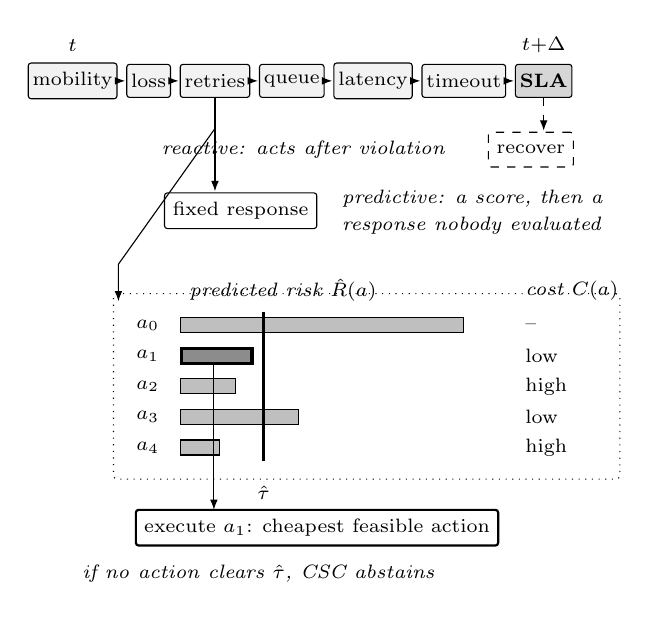
\begin{tikzpicture}[
  font=\footnotesize, x=0.97mm, y=0.97mm,
  chain/.style={draw, rounded corners=1pt, minimum height=4.2mm,
                inner xsep=1.6pt, fill=black!5, font=\scriptsize},
  lbl/.style={font=\scriptsize\itshape},
  note/.style={font=\scriptsize},
  box/.style={draw, rounded corners=1pt, minimum height=4.4mm, inner xsep=3pt,
              font=\scriptsize},
  ar/.style={-{Latex[length=1.3mm]}, shorten >=0.4pt},
  bar/.style={draw, fill=black!25, minimum height=1.9mm, inner sep=0pt, anchor=west},
  barsel/.style={draw, very thick, fill=black!45, minimum height=1.9mm,
                 inner sep=0pt, anchor=west}
]
%--- degradation chain -------------------------------------------------------
\node[chain] (c1) at (2,0) {mobility};
\node[chain, right=1.1mm of c1] (c2) {loss};
\node[chain, right=1.1mm of c2] (c3) {retries};
\node[chain, right=1.1mm of c3] (c4) {queue};
\node[chain, right=1.1mm of c4] (c5) {latency};
\node[chain, right=1.1mm of c5] (c6) {timeout};
\node[chain, right=1.1mm of c6, fill=black!16] (c7) {\textbf{SLA}};
\foreach \s/\d in {c1/c2,c2/c3,c3/c4,c4/c5,c5/c6,c6/c7} \draw[ar] (\s)--(\d);
\node[lbl, above=0.2mm of c1] {$t$};
\node[lbl, above=0.2mm of c7] {$t{+}\Delta$};

%--- reactive ----------------------------------------------------------------
\node[box, dashed] (rec) at (62,-9) {recover};
\draw[ar, dashed] (c7.south) -- (c7.south|-rec.north);
\node[lbl, anchor=east] at (52,-9) {reactive: acts after violation};

%--- predictive --------------------------------------------------------------
\node[box] (fix) at (24,-17) {fixed response};
\draw[ar] (c3.south) -- (c3.south|-fix.north);
\node[lbl, anchor=west] at (36,-15.4) {predictive: a score, then a};
\node[lbl, anchor=west] at (36,-19.0) {response nobody evaluated};

%--- CSC: shadow futures -----------------------------------------------------
\draw[ar] (c3.south) -- ++(0,-4) -- (8,-24) -- (8,-29);
\node[lbl, anchor=west] at (16,-27.4) {predicted risk $\hat{R}(a)$};
\node[lbl, anchor=west] at (60,-27.4) {cost $C(a)$};
\foreach \nm/\yy/\len/\cc in {%
  0/-32/36/{--}, 1/-36/9/{low}, 2/-40/7/{high},
  3/-44/15/{low}, 4/-48/5/{high}}{
  \node[lbl, anchor=east] at (14.6,\yy) {$a_{\nm}$};
  \node[bar, minimum width=\len mm] at (16,\yy) {};
  \node[note, anchor=west] at (60,\yy) {\cc};
}
\node[barsel, minimum width=9mm] at (16,-36) {};
\draw[very thick] (27,-30.2) -- (27,-49.8);
\node[lbl, anchor=north] at (27,-51.8) {$\Rsafe$};
\node[box, thick] (sel) at (34,-58.5) {execute $a_1$: cheapest feasible action};
\draw[ar] (20.5,-37.2) -- (20.5,-56.3);
\node[lbl, anchor=west] at (2,-64.5) {if no action clears $\Rsafe$, CSC abstains};
\begin{scope}[on background layer]
  \node[draw, dotted, rounded corners=1.5pt, inner sep=1.6mm,
        fit={(9,-29.5) (72,-50.5)}] {};
\end{scope}
\end{tikzpicture}

\caption{Reactive, predictive and counterfactual control on the same
degradation chain. Reactive control acts after the SLA is broken; predictive
control acts on a risk score with a fixed response; CSC evaluates the risk of
every candidate action before acting, executes the cheapest action whose
score is admitted by the calibrated gate $\Rsafe$, and abstains when none is.}
\label{fig:concept}
\end{figure}

%==============================================================================
\section{System Model and Counterfactual Shadow Control}

\subsection{System and state}
The system comprises IoT devices $\mathcal{D}=\{d_1,\dots,d_N\}$, edge nodes
$\mathcal{E}=\{e_1,\dots,e_M\}$ and services $\mathcal{V}=\{v_1,\dots,v_K\}$.
Devices move, associate with gateways, and generate events; gateways queue,
retry and route them to edge nodes that execute services subject to an agreement
on end-to-end latency and delivery ratio. The controller observes
\begin{equation}
S_t=(G_t,X_t),\qquad
X_t\in\mathbb{R}^{|\mathcal{N}_t|\times d\times W},
\label{eq:state}
\end{equation}
where $G_t$ is the dependency graph over device, gateway, link, edge-node,
broker and service vertices and $X_t$ stacks $d$ network, edge, application and
mobility features per vertex over a window of $W$ samples. Mobility features
include a link-quality score $q_t\in[0,1]$, an abstract quantity driving network
impairment; it is not a measured radio signal-to-interference-plus-noise ratio
and is not treated as one. The failure event $F_{t+\Delta}$ indicates an
agreement violation sustained within the horizon $\Delta$. The action set is
deliberately small,
\begin{equation}
\Aset=\{a_0,\,a_1,\,a_2,\,a_3,\,a_4\},
\label{eq:actions}
\end{equation}
denoting no action, reroute, workload migration, source throttling and replica
activation --- each a primitive the runtime executes on a live system with
bounded, measurable side effects.

\subsection{Observational and interventional risk}
A temporal predictor $f_\theta$ over graph-aggregated features gives the
observational risk $R^{\mathrm{obs}}(S_t)=\Pr[F_{t+\Delta}=1\mid S_t]
=f_\theta(S_t)$, which is what prediction-only controllers act on. It is not
what CSC acts on, and the two quantities occupy separate fields of the decision
record throughout.

Causal structure is fixed from system semantics rather than discovered, and it
is dynamic: each endogenous variable is generated one tick ahead from its
parents, the action in force, and exogenous noise,
\begin{equation}
X_{j,t+1}=g_j\!\left(\mathrm{Pa}_j(X_t),\,A_t,\,u_{j,t}\right).
\label{eq:scm}
\end{equation}
The parent sets encode mechanisms the deployed system implements ---
$\textit{Mob}\!\to\!\textit{LinkQ}\!\to\!\textit{Loss}\!\to\!\textit{Retry}
\!\to\!\textit{Queue}\!\to\!\textit{Lat}\!\to\!\textit{Timeout}\!\to\!F$, with
$\textit{EvRate}\!\to\!\textit{Queue}$ and
$\textit{Load}\!\to\!\textit{ProcTime}\!\to\!\textit{Queue}$ --- and reverse
edges are excluded on physical grounds, since queue depth at $t$ cannot
influence mobility at $t-1$. This trades discovery generality for
identifiability, supported by evidence that discovered structures transfer
poorly from synthetic data to running systems \cite{pham2024rca}. Structure is
fixed; each $g_j$ is estimated from training observations.

An action replaces the mechanisms it controls. Rerouting is a
\emph{compute-path} intervention: it changes the gateway-to-edge assignment and
therefore the load, queue and processing terms
$g_{\textit{Queue}}$ and $g_{\textit{ProcTime}}$, while leaving link quality and
loss to mobility and the network, which no choice of edge can alter. Migration
replaces the placement term in $g_{\textit{ProcTime}}$, throttling the source
term in $g_{\textit{EvRate}}$, and replication the capacity term in
$g_{\textit{Queue}}$. Writing $\mathcal{M}_a$ for the resulting model, the
interventional risk follows from rolling \eqref{eq:scm} forward
$H=\Delta/\Delta_{\mathrm{tick}}$ steps under $\mathrm{do}(A_t=a)$ and averaging
over sampled noise:
\begin{equation}
R(a\mid S_t)=\Pr\nolimits_{\mathcal{M}_a}\!\left[\textstyle\bigcup_{h\le H}
\{F^{a}_{t+h}=1\}\;\middle|\;\mathrm{do}(A_t=a),\,S_t\right].
\label{eq:int}
\end{equation}
Identification requires that \eqref{eq:scm} contain no unmeasured common cause
of an intervened variable and $F$, and that unintervened mechanisms be invariant
to the intervention. Reliance on the first is weakened by construction rather
than by assumption: at training anchors every action is executed in its own
branch, so the mechanisms are fitted on transitions
$(S_t,a,S^{a}_{t+1},Y^{a})$ in which assignment was forced rather than chosen,
for all $a$ and not one sampled action. This is a designed experiment on the
emulator, and it removes the need for propensity weighting. Training,
calibration and test anchors come from disjoint seed blocks, and test branch
outcomes are visible to no model.

\subsection{Intervention cost}
Each action carries a normalised cost
\begin{equation}
C(a)=w_L\hat{L}_a+w_R\hat{E}_a+w_B\hat{B}_a+w_D\hat{D}_a,
\qquad \textstyle\sum w=1,
\label{eq:cost}
\end{equation}
over added latency, resource use, bandwidth overhead and disruption, each
normalised by the range observed during calibration and clipped to $[0,1]$,
$\tilde{x}=\mathrm{clip}\!\left((x-x^{\mathrm{cal}}_{\min})/
(x^{\mathrm{cal}}_{\max}-x^{\mathrm{cal}}_{\min}),0,1\right)$. Clipping is not
cosmetic: under scenario shift a component can exceed the calibration range, and
an unclipped cost above one would silently reweight the objective on exactly the
runs where the method is under most strain. Degenerate ranges are handled as
documented in the supplement. Equal weights are fixed a priori in version
control as a neutral default, before any comparative result is examined;
sensitivity to alternative operational preferences is reported separately.

\subsection{Uncertainty-filtered, risk-calibrated admissible set}
\label{sec:gate}
Two different things happen at the gate, and conflating them would misstate what
is guaranteed. Actions are first \emph{filtered} by an uncertainty estimate that
is not itself calibrated, and the surviving threshold is then \emph{calibrated}
against a declared risk level.

\textbf{Uncertainty.} $\hat{U}$ is epistemic disagreement among bootstrap
replicas of the structural model. Fitting $B$ replicas $\mathcal{M}^{(1)},\dots,
\mathcal{M}^{(B)}$ on resampled training runs and rolling each forward under
$\mathrm{do}(A_t=a)$ gives $\hat{R}_b(a\mid S_t)$, and
\begin{equation}
\hat{U}(a\mid S_t)=Q_{0.95}\!\left\{\hat{R}_b(a\mid S_t)\right\}
-Q_{0.05}\!\left\{\hat{R}_b(a\mid S_t)\right\},
\label{eq:unc}
\end{equation}
a quantile width rather than a standard deviation, so that a few divergent
replicas do not dominate. $B$ and $U_{\max}$ are selected on the
\emph{validation} split alone and frozen before calibration begins; neither is
touched by calibration or test data. A $5$--$95$ interval estimated from a small
ensemble sits on its extreme order statistics, so $B$ is chosen in the pilot
from $\{20,30,50\}$ on the stability of $\hat{U}$ and of the induced ranking,
against inference overhead.

\textbf{Admissible set.} With $\tau$ a threshold on predicted risk,
\begin{equation}
\Asafe(\tau)=\left\{a\in\Aset \;:\; \hat{R}(a\mid S_t)\le\tau
\;\wedge\; \hat{U}(a\mid S_t)\le \Umax\right\}.
\label{eq:feasible}
\end{equation}
A point estimate of \eqref{eq:int} does not authorise a change to a running
system, and it is not a calibrated probability. We do not conformalise
$R(a\mid S_t)$: it is latent, and a replayed branch yields a binary outcome
rather than that probability, so the residuals split conformal prediction
requires do not exist. The threshold is calibrated instead.

\textbf{Calibration unit.} Decision points inside one run are temporally
dependent and are not exchangeable samples. The unit is therefore an
\emph{independent calibration run}: for run $i$ with a pre-declared anchor set
$\mathcal{T}_i$,
\begin{equation}
L_i(\tau)=\frac{1}{|\mathcal{T}_i|}\sum_{t\in\mathcal{T}_i}
\mathbf{1}\!\left[\exists\,a\in\Asafeit(\tau):\;Y^{a}_{it}=1\right],
\label{eq:loss}
\end{equation}
the within-run rate of admissible sets containing a failure-inducing action,
where $Y^{a}_{it}\in\{0,1\}$ is observed by executing $a$ in its replay branch.
$L_i$ is bounded in $[0,1]$ and non-decreasing in $\tau$, being a mean of
indicators that are individually non-decreasing, which is what conformal risk
control requires \cite{angelopoulos2024crc}. Independent seeds alone do not make
runs exchangeable, however: the calibration runs are drawn from a declared
generating distribution $P_{\mathrm{ID}}$ over scenario, severity, workload and
seed, and the identically distributed test runs are drawn independently from the
same $P_{\mathrm{ID}}$ with disjoint seeds. Scenario shift lies outside
$P_{\mathrm{ID}}$ by construction.

\textbf{Threshold selection.} With $n$ calibration runs, empirical risk
$\hat{L}_n(\tau)=n^{-1}\sum_i L_i(\tau)$ and loss bound $B_\ell=1$, the
finite-sample rule of \cite{angelopoulos2024crc} takes the \emph{largest}
admissible threshold,
\begin{equation}
\hat{\tau}=\sup\left\{\tau:\;
\frac{n\hat{L}_n(\tau)+B_\ell}{n+1}\le\delta\right\},
\label{eq:crc}
\end{equation}
giving $\mathbb{E}[L_{n+1}(\hat{\tau})]\le\delta$ over a future run drawn from
$P_{\mathrm{ID}}$. The largest threshold is taken because $\Asafe$ grows with $\tau$: among
thresholds meeting the risk constraint, the widest admissible set leaves the
cost rule the most room. Selecting $\tau$ by uncorrected empirical risk would
not carry the guarantee, and the correction is not optional at $n=20$--$30$
runs.

\textbf{What is and is not claimed.} Whenever $\Asafe$ is non-empty, the failure
indicator of \emph{any} admissible action it contains is pointwise dominated by
$\ell$, so \eqref{eq:crc} also bounds the \emph{expected within-run failure
rate} of any rule selecting from that set --- including the cost rule below.
That is what makes the guarantee survive the controller choosing adaptively
after seeing all five scores. It concerns the expected within-run rate over
future runs drawn from $P_{\mathrm{ID}}$, not individual decision points; it is
neither per-decision nor conditional, and it says nothing about the latent
$R(a\mid S_t)$. It also does not cover abstention: when
$\Asafe(\hat\tau)=\emptyset$ the loss in \eqref{eq:loss} is zero by
construction, whatever the fallback then does, so fallback rate and fallback
failure rate are measured and reported separately rather than folded into the
guarantee. Finally, $\hat\tau$ is calibrated offline and \emph{frozen}: updating
it online would require the outcomes of actions the running system did not take,
which only a reconstructible environment can supply. Under scenario shift the
frozen $\hat\tau$ is carried over, exchangeability fails by construction, and we
report realised empirical risk against the nominal $\delta$ instead of a
guarantee.

\subsection{Minimum-necessary intervention}
The controller takes the cheapest admissible action rather than the safest:
\begin{equation}
a^{*}_t=
\begin{cases}
\displaystyle\arg\min_{a\in\Asafe(\hat\tau)} C(a), & \Asafe(\hat\tau)\neq\emptyset,\\[6pt]
a_{\mathrm{fb}}, & \Asafe(\hat\tau)=\emptyset .
\end{cases}
\label{eq:mni}
\end{equation}
The first branch says that once predicted risk is admissible, further risk
reduction does not justify further disruption: if rerouting is admitted,
migrating the workload is a more expensive route to a state the system has
already reached. The second is guarded abstention --- with nothing admissible the controller
executes a predetermined fallback rather than the least-bad learned option. We
avoid calling it \emph{safe}: the fallback lies outside \eqref{eq:crc}, which
constrains the admissible set and says nothing about what happens when that set
is empty, so the fallback's own failure rate is measured and reported alongside. This follows the gating principle of \cite{desilva2026aurora}; the
difference is that $\hat\tau$ is calibrated to a declared level, so how often
the gate is wrong is a reported quantity. The controller never falls back to
$\arg\min_a \hat{R}(a)$; that is ablation A2, not the method. After execution it
observes $S_{t+\Delta}$ and records the error
$\epsilon_t=Y_{t+\Delta}-\hat{Y}^{\,a^{*}}_{t+\Delta}$, which drives drift
detection and is reported as calibration decay --- it does not silently move
$\hat\tau$, for the reason given above.

\section{Prototype and Experimental Methodology}
\label{sec:method}

\begin{figure}[!t]
\centering
% Fig. 2 -- prototype architecture.
% Grayscale-safe. Go plane = single border, Python plane = double border.
% Control flow solid, telemetry dashed, closed-loop feedback dotted.
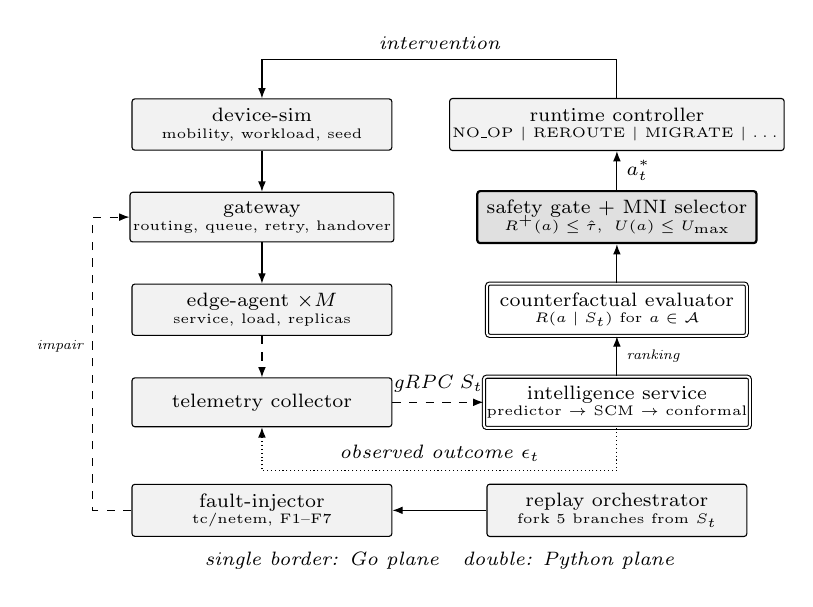
\begin{tikzpicture}[
  font=\footnotesize, x=0.98mm, y=0.98mm,
  go/.style={draw, rounded corners=1pt, minimum height=6.2mm,
             minimum width=33mm, inner xsep=1pt, align=center, fill=black!5,
             font=\scriptsize},
  py/.style={draw, double, double distance=0.7pt, rounded corners=1pt, minimum height=6.2mm,
             minimum width=33mm, inner xsep=1pt, align=center, fill=white,
             font=\scriptsize},
  gate/.style={draw, thick, rounded corners=1pt, minimum height=6.6mm,
               minimum width=33mm, align=center, fill=black!12, font=\scriptsize},
  ar/.style={-{Latex[length=1.3mm]}},
  tel/.style={-{Latex[length=1.3mm]}, dashed},
  fb/.style={-{Latex[length=1.3mm]}, densely dotted},
  lbl/.style={font=\scriptsize\itshape}
]
\node[go] (dev)  at (0,0)    {device-sim\\[-2pt]{\tiny mobility, workload, seed}};
\node[go] (gw)   at (0,-12)  {gateway\\[-2pt]{\tiny routing, queue, retry, handover}};
\node[go] (edge) at (0,-24)  {edge-agent $\times M$\\[-2pt]{\tiny service, load, replicas}};
\node[go] (tel)  at (0,-36)  {telemetry collector};

\node[py]   (intel) at (46,-36) {intelligence service\\[-2pt]{\tiny predictor $\to$ SCM $\to$ conformal}};
\node[py]   (cf)    at (46,-24) {counterfactual evaluator\\[-2pt]{\tiny $R(a\mid S_t)$ for $a\in\Aset$}};
\node[gate] (gate)  at (46,-12) {safety gate $+$ MNI selector\\[-2pt]{\tiny $R^{+}(a)\le \Rsafe$,\; $U(a)\le \Umax$}};
\node[go]   (ctl)   at (46,0)   {runtime controller\\[-2pt]{\tiny NO\_OP $\mid$ REROUTE $\mid$ MIGRATE $\mid\dots$}};

\node[go] (fault) at (0,-50)  {fault-injector\\[-2pt]{\tiny tc/netem, F1--F7}};
\node[go] (rep)   at (46,-50) {replay orchestrator\\[-2pt]{\tiny fork 5 branches from $S_t$}};

\draw[ar]  (dev)  -- (gw);
\draw[ar]  (gw)   -- (edge);
\draw[tel] (edge) -- (tel);
\draw[tel] (tel)  -- node[lbl, above]{gRPC $S_t$} (intel);
\draw[ar]  (intel) -- node[lbl, right]{\tiny ranking} (cf);
\draw[ar]  (cf)   -- (gate);
\draw[ar]  (gate) -- node[lbl, right]{$a^{*}_t$} (ctl);
\draw[ar]  (ctl.north) -- ++(0,5) -| node[lbl, above, pos=0.25]{intervention} (dev.north);
\draw[fb]  (intel.south) -- ++(0,-5.5) -| (tel.south);
\node[lbl] at (23,-42.6) {observed outcome $\epsilon_t$};
\draw[ar, dashed] (fault.west) -- ++(-5,0) |- node[lbl, left, pos=0.28]{\tiny impair} (gw.west);
\draw[ar]  (rep) -- (fault);
\node[lbl] at (23,-56.5) {single border: Go plane\quad double: Python plane};
\end{tikzpicture}

\caption{Prototype architecture. The Go plane owns time, concurrency and every
side effect. The Python plane returns action-conditioned risk scores,
uncertainty estimates and predicted costs, and has no authority to act; the Go
controller applies the frozen $\hat\tau$ and $\Umax$ and selects. A slow or
unavailable intelligence plane therefore produces a recorded fallback rather
than a stalled decision.}
\label{fig:arch}
\end{figure}

\subsection{Implementation}
CSC is a distributed prototype in which a Go plane executes and a Python plane
infers (Fig.~\ref{fig:arch}). The Go services are a device simulator, a gateway
performing routing, queueing, retry, backpressure and handover, edge agents
exposing load, queue depth, service time and replication state, a fault
injector, a replay orchestrator and the controller; the Python service hosts the
predictor, the structural model, the calibrator and the counterfactual
evaluator. The planes communicate over a typed RPC boundary, gateway-to-edge
work and telemetry travel over a message bus; the concrete implementations and
their versions are recorded in every run manifest together with a runtime-stack
identifier, because the replay resolution reported below is a property of one
stack --- transport, kernel, images, process topology --- and does not transfer
to another. Reproducibility rests on an explicit experiment clock
and per-component random streams derived as
$\mathrm{seed}_i=H(\mathrm{master},\,\mathrm{component})$, so that changing one
component's sampling does not perturb another's schedule.

Placing the gate and the selector of \eqref{eq:feasible}--\eqref{eq:mni} in the
Go controller keeps the component that may refuse to act separate from the one
that may be miscalibrated, and makes the decision path an RPC with an enforced
deadline. A deadline miss is recorded as a fallback rather than awaited, which
lets overhead be reported as a bounded cost rather than an average.

\subsection{Testbed and scenarios}
Experiments run on a software-defined emulation testbed rather than a numerical
simulation: real processes, queues, typed RPC calls over TCP, and container
scheduling. Network conditions are emulated with Linux traffic control and
\texttt{netem} on the device simulator's device-network egress, matching the
device-to-gateway direction, driven by the link-quality score; mobility and radio behaviour
are modelled, not measured. Reported results use the privileged kernel path
only; the application-layer impairment path used on unprivileged hosts is
recorded in the manifest and never mixed in.

Edge nodes differ in service capacity by construction: each serves a bounded
number of events per epoch and queues the remainder, and the capacities are
unequal. With identical edges a reroute moves work to a node that behaves the
same way, so the action cannot change any outcome and its measured effect is
zero for a reason that has nothing to do with the controller. Waiting time is
counted in epochs rather than wall-clock seconds, so that an outcome is a
function of the logical schedule rather than of how heavily the host was loaded
while the branch ran. Table~\ref{tab:scenarios} lists the seven scenarios.

Six controllers are compared: a reactive threshold controller (B1); a GRU
predictor with a heuristic recovery rule (B2); a graph predictor with the same
rule (B3); a PPO policy under a pre-declared reward (B4)
\cite{schulman2017ppo}; CSC-Predict (B5), which estimates
$\hat{\Pr}(F_{t+\Delta}\mid S_t, A_t\!=\!a)$ with the action supplied as an
ordinary predictor input and performs no structural intervention; and CSC (B6).
B5 is the load-bearing comparison: it asks whether the structural model and
$\mathrm{do}(a)$ buy anything over a supervised action-conditioned predictor
given the same training information. All learned controllers share features,
windows, action set, execution mechanism and hyperparameter budget, and none
sees future information or replay outcomes. Three ablations remove the
calibrated gate, minimum-necessary selection (reverting to
$\arg\min_a \hat R(a)$), and the structural layer.

\subsection{Replay-based reference outcomes}
At recorded decision points the run is reconstructed from a deterministic
prefix specification --- master seed, per-component streams, configuration,
workload and fault schedules, and the action history up to $t$ --- and
re-executed with only the action at $t$ replaced. The \emph{inputs} are
reproduced exactly; the concurrent execution schedule is not, and the residual
nondeterminism this leaves is measured rather than assumed away. We reconstruct rather than snapshot: congestion
windows, goroutine schedules, broker buffers and in-flight packets cannot be
captured faithfully. Each anchor carries
$\mathrm{sid}=\mathrm{SHA256}(\text{config}\|\text{seed}\|t\|\text{history})$
and each branch $\mathrm{bid}=(\mathrm{sid},a)$.

We call the results \emph{replay-based empirical reference outcomes}, not
counterfactual ground truth: the system is concurrent and residual
nondeterminism remains.

Branches are taken only at logical epoch boundaries, and a component reporting
that it finished the preceding tick is not sufficient evidence that the epoch is
over: on an asynchronous bus a message published during that tick may still be
in flight. Each producer therefore declares its last sequence number for the
epoch and each consumer confirms consumption through it, so the anchor opens
only once the transport itself is drained. A branch set is then aborted unless
both the transport watermarks and the structural state match the anchor's
\emph{exactly}. The structural state covers all future-relevant discrete state
--- queue \emph{content} digests rather than depths alone, retry sets with
attempt counts and backoff deadlines in logical time, current rate-limiter
tokens rather than configured limits, timeout deadlines, routing and service
placement, replica and pending-migration state, fault phase, processed sequence
positions and action history. Two queues of equal depth holding different events
have different futures, and admitting any tolerance would let pre-action state
mismatch enter the dispersion band and inflate it with its own imprecision. A separate audit (D0) then re-executes a fixed set
of anchors under the \emph{same} action many times and estimates
$\eta_J=Q_{0.95}(|J_{r_i}(a)-J_{r_j}(a)|)$; two actions count as
distinguishable only when their observed objectives differ by more than
$\eta_J$. $\eta_J$ is a property of one runtime stack --- transport, container
images, kernel and process topology --- and is invalidated by a change to any of
them.

The intervention itself is acknowledged. After recording the anchor, the target
component returns a run-scoped acknowledgement containing the action identifier
only after its routing or admission state has changed; the orchestrator refuses
a branch that reaches the next epoch without this evidence.

Predicted and observed objectives are kept strictly separate. The controller
ranks with $\hat{J}(a)=\lambda_F\hat{R}(a)+\lambda_L\hat{L}(a)
+\lambda_C\hat{C}(a)$, whereas the reference objective is computed only from what
the branch did:
\begin{equation}
J^{\mathrm{obs}}(a)=\lambda_F Y^{a}+\lambda_L\tilde{L}^{a}
+\lambda_C C^{a}_{\mathrm{obs}}.
\label{eq:jobs}
\end{equation}
No model output enters \eqref{eq:jobs}; if it did, the reference ranking would
contain the prediction it is meant to test. In the deployed testbed $Y^{a}$ is
the share of offered work that violated the latency budget or remained unserved
at the horizon, $\tilde{L}^{a}$ the mean waiting time normalised by a
calibration maximum fixed before the comparison, and $C^{a}_{\mathrm{obs}}$ the
realised cost of the action. The cost term is currently populated from measured
disruption --- work deferred or displaced by the action --- while the resource
and bandwidth components of \eqref{eq:cost} are not yet instrumented; runs
computed on that reduced term are reported as such and the analysis refuses to
emit \eqref{eq:jobs} silently without them. Ranking quality and regret follow,
with ties resolved by $\eta_J$:
\begin{align}
\mathrm{CRA}_\eta&=\frac{1}{|\mathcal{T}|}\sum_{t\in\mathcal{T}}
\mathbf{1}\!\left[J^{\mathrm{obs}}_t(a^{*}_t)\le
\min_{a}J^{\mathrm{obs}}_t(a)+\eta_J\right],
\label{eq:cra}\\
\mathrm{Reg}_\eta(t)&=\max\!\left(0,\;J^{\mathrm{obs}}_t(a^{*}_t)
-\min_{a}J^{\mathrm{obs}}_t(a)-\eta_J\right).
\label{eq:regret}
\end{align}
Replay records are quarantined from every training set and a leakage test fails
the build if one appears.

\subsection{Two evaluation layers}
Controllers that intervene change the trajectory, so after the first divergent
action they no longer face the same decision points. Comparing them on a metric
whose denominator is controller-specific --- the set of preventable failures each
one happened to encounter --- would not be an equal comparison. Evaluation is
therefore split.

The \emph{common-anchor decision benchmark} presents every decision method with
the \emph{same} replayed anchors, drawn from a reference trajectory, and asks
whether it chose well: $\mathrm{CRA}_\eta$, $\mathrm{Reg}_\eta$, and
common-anchor PFR and WIR, all on a shared denominator. The \emph{closed-loop
benchmark} lets each controller run end to end and diverge, and asks whether
those choices improved the system: availability, agreement-violation rate,
failure count, tail latency, intervention cost, resource use, and
abstention and fallback rates. The first isolates decision quality, the second
measures system outcome, and neither substitutes for the other.

\subsection{Metrics and protocol}
On common anchors, write $N_{\mathrm{pre}}$ for the decision points where the no-action branch
failed \emph{and} some alternative branch did not --- excluding failures no
available action could have averted --- $N_{\mathrm{prev}}$ for those where the
no-action branch failed and the executed action's branch did not, $N_{\mathrm{int}}$
for the interventions taken, and $N_{\mathrm{harm}}$ for those whose branch
objective exceeded the no-action branch by more than $\eta_J$. Then
\begin{equation}
\mathrm{PFR}=N_{\mathrm{prev}}/N_{\mathrm{pre}},
\qquad
\mathrm{WIR}=N_{\mathrm{harm}}/N_{\mathrm{int}}.
\label{eq:pfr}
\end{equation}
Both rest on executed alternatives rather than on a model's opinion of them, and
both are reported on the common-anchor layer where the denominator is shared.
Failure lead time, availability, violation rate, mean intervention cost, tail
latency, abstention rate, fallback rate and fallback failure rate are reported
on the closed-loop layer. Decision overhead
$T_{\mathrm{dec}}=T_{\mathrm{feat}}+T_{\mathrm{rpc}}+T_{\mathrm{model}}
+T_{\mathrm{cf}}+T_{\mathrm{gate}}$ is reported at the $95$th percentile with
the deadline-miss rate rather than as a median. The transport term is separated
because the intelligence plane is a distinct process: folding serialisation and
network time into the model term would hide where a missed deadline came from.
$T_{\mathrm{cf}}$ scales with $|\Aset|$ and the horizon $H$. Predictive metrics are secondary; accuracy is not reported, the
positive class being rare by construction.

Data are split by run, never by row: training, validation and calibration draw
disjoint seed blocks from F1--F4, the identically distributed test set uses new
seeds \emph{and} new parameter values within F1--F4, and F5--F7 and combined
faults are held out entirely as scenario shift, used for no selection decision.
Every controller runs against the same seed-specific realisation, so comparisons
are paired over at least $20$ seeds, with bootstrap intervals, paired Wilcoxon
tests, effect sizes and Holm correction. The availability claim for
minimum-necessary intervention is a non-inferiority claim, tested as one against
a pre-declared margin rather than inferred from a non-significant difference.
The pre-registered protocol, exclusion policy, configurations and per-seed
observations ship with the artifact.

% Table II -- scenarios. Values mirror experiments/scenarios/F*.yaml.
% If a value here disagrees with the YAML, the YAML is right and this is a bug.
\begin{table}[!t]
\caption{Failure Scenarios and Their Parameters}
\label{tab:scenarios}
\centering
\footnotesize
\setlength{\tabcolsep}{3.5pt}
\begin{tabular}{@{}llll@{}}
\toprule
ID & Scenario & Driving parameter & Split \\
\midrule
F1 & Gradual link degradation & loss $0\to20\%$ over $120$\,s      & train / ID \\
F2 & Latency inflation        & RTT $10\to250$\,ms                 & train / ID \\
F3 & Edge compute overload    & load $0.3\to0.95$                  & train / ID \\
F4 & Queue congestion         & $\lambda>\mu$, ratio $1.5\times$   & train / ID \\
F5 & Mobility with handover   & gateway reassociation              & \textbf{shift} \\
F6 & Abrupt node failure      & edge node terminated               & \textbf{shift} \\
F7 & Cascading failure        & F5 $\to$ loss $\to$ retry $\to$ queue & \textbf{shift} \\
\bottomrule
\end{tabular}
\\[2pt]
{\footnotesize F1--F4 constitute $P_{\mathrm{ID}}$; F5--F7 are held out entirely.}
\end{table}


%==============================================================================
\section{Results}
\label{sec:results}

Results are reported in the order in which they became interpretable. The
measurement is established first, then replay resolution, then what the actions
do, and only then what can be predicted about them. Nothing below is typed by
hand: every figure is emitted by \texttt{analysis/make\_tables.py} from the
recorded runs, and each table names the run, the runtime stack and the protocol
revision that produced it.

Two of the four completed matrices are \emph{not} reported. Their objective was
computed from observables that did not mean what the analysis assumed, the
defects and their dated corrections are in the protocol's amendment log, and the
runs are superseded rather than reinterpreted. What follows comes from the two
runs that pass the accounting audit described next.

\subsection{The measurement is audited before it is interpreted}
\label{sec:results-audit}

Every branch is checked against seven accounting invariants: that the numerator
and the denominator of the objective cover one set of events; that eligible
unserved work is a subset of the queue; that every served event appears exactly
once in the latency histogram; that violations are a subset of served work; that
the histogram agrees with the violation count at the frozen budget; that only a
throttled branch defers work at the gateway; and that a branch spanning no fault
fails nothing. A violation of any of these is an instrumentation defect and
never a property of the system, so a run that fails them is not reported.

A further invariant checks that the declared fault had an \emph{effect} rather
than merely being configured: an edge whose capacity drops to $S$ at epoch $T$
cannot have served more than $N(T-1) + S(H-T+1)$ events, whatever the action.
The bound is one-sided, because serving less is ordinary --- rerouting moves work
away and an unsaturated node serves only what arrives --- so only the upper limit
carries information. On the scenario-factored matrix it binds on 2175 of 2880
branches and holds on all of them.

Both reported runs pass all invariants on every branch, with no refused branch
and prefix identity holding within every replay cell.

\subsection{Determinism and replay resolution}
\label{sec:results-replay}

\input{generated_tables/table_bands_single.tex}

Table~\ref{tab:bands-single} reports the replay dispersion band before any
comparison that depends on it. The preregistered definition is the pooled
$Q_{0.95}$ of within-cell differences, and that figure resolves 45 of 60 action
contrasts at the gate. The band is not uniform, however: the worst single cell is
$2.8\times$ the pooled value, and the protocol states that a band holding on
average while failing in one cell is not a band. We therefore report the gate
under four bands and name the set that survives all of them --- 33 of 60
contrasts. The preregistered number is the one the hypothesis was stated against;
the four-band set is what can be claimed without depending on which band is
chosen.

The dispersion is dominated by the failure term, which carries $89\%$ of it.
This is a property of the instrument rather than of the system: service occurs on
epoch boundaries and events are emitted across a window, so per-event latency in
a healthy system spreads by roughly that window and a budget placed inside the
spread measures emission phase rather than failure. The budget is therefore
calibrated by a declared rule --- the healthy per-event $p_{99}$, rounded up to
50\,ms, measured on a dedicated no-action calibration run at the same offered
load --- and frozen before any comparison. At the calibrated 750\,ms, $0.9\%$ of
a healthy system's events exceed it. An earlier budget of 500\,ms, derived from
branch-mean rather than per-event latency, classified $31\%$ of a working
system's events as failures.

\subsection{What the actions do}
\label{sec:results-actions}

Three findings survive the four-band criterion, and they are reported with their
regime, because the regime is what makes them interpretable. A branch is
\emph{pre-fault} when its horizon ends before the fault onset, \emph{spanning}
when the onset falls inside the horizon, and \emph{post-onset} when the fault is
already running at the anchor. The labels are computed from each branch's own
numbers rather than from its position in the design.

First, intervening in a system that is not degrading does nothing. At the
pre-fault anchors the contrast between no action and rerouting is $0.000$ with a
bootstrap interval of $[-0.000, +0.005]$. This is a measured null rather than a
failure to resolve, and it is the empirical content of minimum-necessary
intervention: the mechanism declines to act when there is nothing to act on.

Second, throttling is harmful wherever it is resolvable, and most harmful
earliest. It is the clearest effect in the data --- at the shallowest anchors its
signal exceeds the band by more than an order of magnitude --- and it becomes
indistinguishable from inaction at the deepest anchors not because it stops
hurting but because inaction has caught up with it.

Third, the value of intervening decays with delay. The no-action-minus-reroute
contrast rises to $0.264$ at an intermediate anchor and falls to $0.174$ at the
deepest one, with non-overlapping bootstrap intervals at the two ends. The same
ordering appeared in every run of this design, at two different latency budgets
and under two different definitions of the objective's denominator, which is the
strongest evidence available here that it is a property of the system rather than
of the instrument.

\subsection{What decision-time telemetry predicts}
\label{sec:results-prediction}

\input{generated_tables/table_bands_factored.tex}
\input{generated_tables/table_prediction.tex}

The single-scenario run cannot support any claim about generalisation: one fault
onset and one severity make the anchor index an exact proxy for how long the
fault has been running, so a predictor could score well by memorising a schedule
that never varies. The fault is therefore a declared factor --- onset, severity,
offered load and seed are drawn per scenario and held fixed within a replay cell
and across the actions compared at an anchor --- and prediction is evaluated with
folds held out by fault design point, so that no test scenario shares its fault
setting with any training scenario.

Table~\ref{tab:prediction} reports an action-conditioned predictor of
$J_{\mathrm{obs}}$ built only from state observable at the decision instant. The
feature set provably excludes the fault schedule: onset, severity, mechanism and
the node's reported degradation configuration are forbidden by name and by
substring, and the exclusion is tested by rewriting the recorded schedule in a
copy of the anchor state and asserting that the feature vector is unchanged. What
the model may see is the observable trace of degradation --- throughput below the
node's nominal capacity, queue depth, the latency distribution so far.

Two controls decide whether the result means anything. A time-only predictor
given the elapsed epoch and the candidate action reaches $0.1174$; the telemetry
model reaches $0.0261$, cutting the error by $78\%$, so the skill is not the
clock. Permuting the telemetry between branches while leaving actions and targets
in place raises the error to $0.1607$, a factor of $6.2$, so the skill comes from
the telemetry rather than from anything else in the design. Both controls are
required to pass before any prediction figure is reported, and the table is not
generated otherwise.

The per-regime rows qualify the headline. The pre-fault regime is the easiest and
the least informative, because $J_{\mathrm{obs}}$ is nearly constant there by
construction. The spanning regime is the interesting one: the fault has not
happened at decision time and nothing in the observed state carries it, yet the
error is far below a constant. Two explanations fit, and they mean opposite
things. Either the model reads what has already accumulated, in which case the
skill would exist in a deployment; or it has learned this experiment's
distribution of onsets from other branches that span faults, in which case it
would not.

\input{generated_tables/table_spanning.tex}

Table~\ref{tab:spanning} separates them. Removing every spanning branch from
training, and additionally every branch sharing the test branch's fault setting,
leaves the error at $0.0479$ against $0.1922$ for a constant --- a factor of
four, and only $1.4\times$ worse than when spanning examples are allowed. The
skill therefore transfers: it comes from the observed state rather than from
knowledge of when faults arrive in this design.

That result also bounds what the method can claim. The strict error in the
spanning regime is $1.9\times$ the error where the fault is already running, and
the residual is the part of the outcome that the arrival of an unobserved fault
decides. No predictor built on this state can remove it, and the paper does not
suggest that conformal calibration does: the guarantee is over the observed
distribution, and an event absent from the observations lies outside it.

\subsection{What the structural model needs from the telemetry}
\label{sec:results-identifiability}

The structural predictor $\hat{J}(s,a)$ is queueing arithmetic with no fitted
parameters: it advances the admission backlog and the per-edge queues over the
planning horizon under the semantics of the action, takes the shape of the
per-event latency distribution as measured and computes only its shift, and then
scores the result with the same objective, over the same branch-level window, as
the measurement. It was written and frozen before the associative challenger was
evaluated, and its acceptance test was fixed in the protocol in advance: it must
reproduce the \emph{sign} of every contrast the measurement can resolve, that is
every contrast surviving all four bands of Section~\ref{sec:results-actions}.
Direction, not magnitude, is what a controller consumes.

Built on cumulative counters, the model fails that test, and the failure is
informative. Let $\lambda$ be the offered rate, $c$ the effective service rate
and $k$ the epoch index. Cumulative served work and current queue depth satisfy
$\mathrm{served} + q = \lambda k$ identically, so no function of them separates
the onset of a degradation from its severity: only the product of depth and
duration is observable. A direct test confirms this. Estimating capacity as
$q/w_{\max}$ over 104 post-onset no-action branches gives medians $103.3$,
$100.0$ and $83.3$ for declared post-fault capacities of $40$, $60$ and $90$ ---
it recovers the arrival rate, near $100$, and not the capacity. The cumulative
throughput $\mathrm{served}/k$ does order with severity ($67.8$, $78.7$, $91.7$)
but is biased upward, because it averages healthy and degraded epochs.

The same absence defeats the arrival rate. Of $203$ resolvable contrasts the
frozen model reproduced $190$ signs; all $13$ failures were the admission-cap
action at the earliest anchor, where the observed contrast is near $-0.67$ and
the prediction near zero. At epoch two the cumulative arrival rate reads $50$
because it still contains the warm-up ramp, while the steady rate is $100$; an
admission cap of $50$ therefore appears not to bind when in fact it binds hard.
In the post-onset regime, where the ramp is long past, the model reproduced
$103$ of $103$ signs.

We report this as a requirement on instrumentation rather than as a defect of
the model. A decision-time state built from cumulative counters is not
sufficient for structural reasoning about capacity, however the model is
written; a windowed rate --- work served and work admitted in the last completed
interval --- is standard in production telemetry and restores identifiability of
the current operating point. Each node now reports both. The objective, the
resolvability gate, the bands and the retention rule are unchanged, and the
pre-amendment predictions and sign test are retained in the artifact so that the
sequence can be audited.

\subsection{Structural versus associative prediction}
\label{sec:results-b5}
\TODO{The comparison that decides the architecture. Report
$\mathrm{CRA}_\eta$ and $\mathrm{Reg}_\eta$ for the structural model and the
associative challenger in three regimes --- in-distribution, parameter shift and
mechanism shift --- and apply the retention rule fixed in the protocol before
these test sets were inspected. A tie is reported as a tie.}

\subsection{Common-anchor decision quality}
\TODO{$\mathrm{CRA}_\eta$, $\mathrm{CRA@2}$, $\mathrm{Reg}_\eta$, and
common-anchor PFR and WIR, all on the shared denominator, for every decision
method including the shifted anchors of F5--F7. This subsection carries H1 and
H2; report them including if they fail.}

\subsection{Closed-loop system outcome}
\TODO{Availability, violation rate, failure count, p99 latency, intervention
cost, abstention and fallback rates on diverging trajectories. State plainly
where decision quality did and did not translate into system outcome --- that
gap, if it exists, is a finding, not an embarrassment.}

\input{generated_tables/table_main.tex}

\subsection{Risk control under scenario shift}
\TODO{Realised within-run set-level risk against the nominal $\delta$ on ID and
shifted scenarios, with abstention, fallback and fallback-failure rates. On ID
this tests \eqref{eq:crc} directly; on F5--F7 exchangeability is violated by
construction and only the empirical figure is reported. Report degradation where
it occurs.}

\begin{figure}[!t]
\centering
\TODO{fig3\_timeline.pdf --- cascading-failure timeline: degradation onset,
predicted no-action counterfactual, intervention point, observed outcome.}
\caption{Cascading failure (F7): observed degradation, the counterfactual
no-action trajectory obtained by replay, the intervention point, and the
realised recovery.}
\label{fig:timeline}
\end{figure}

\subsection{Ablations}
\TODO{A1 no gate, A2 no minimum-necessary intervention, A3 no causal layer.
A2 is the load-bearing one for H3: it isolates cost reduction from risk
reduction.}

\input{generated_tables/table_ablation.tex}

\subsection{Overhead and scalability}
\TODO{Decomposition of $T_{\mathrm{dec}}$, CPU and memory, and the curve from
100 to 10{,}000 devices. Report $p_{95}$ and the deadline-miss rate against the
declared budget, not the median. State the largest device count actually run; do
not extrapolate.}

\begin{figure}[!t]
\centering
\TODO{fig4\_main.pdf --- 2$\times$2 panel: PFR, WIR, p99 latency, mean
intervention cost across controllers.}
\caption{Primary comparison across controllers. Bars show means with $95\%$
bootstrap confidence intervals over paired seeds.}
\label{fig:main}
\end{figure}

%==============================================================================
\section{Discussion and Limitations}
\label{sec:discussion}

The structure in \eqref{eq:scm} is asserted from system semantics, and
identification of \eqref{eq:int} rests on the absence of unmeasured common
causes and on the invariance of unintervened mechanisms. Reliance on
observational assignment is reduced by exhaustive interventional training
branches --- every candidate action is executed from every training anchor, so
assignment is forced rather than chosen --- which improves action coverage but
removes neither structural misspecification nor the invariance assumption. What is checkable is whether the resulting rankings agree with
executed alternatives, which is what \eqref{eq:cra} and \eqref{eq:regret}
measure: a structure wrong in a way that matters should surface there rather
than hide behind good predictive scores.

The evaluation runs nine containers on a single host. No claim is made about
geographic distribution, multi-host placement or multi-tenancy, and none can be
supported by this substrate; what the substrate supports is a claim about the
decision procedure and about how its effect is measured, both of which are
independent of where the containers run. The cost term is reduced: it carries
displaced and undelivered work, while the resource and bandwidth components
named in Section~\ref{sec:results} are not instrumented, and every table
reporting $J_{\mathrm{obs}}$ says so. Two of the four completed matrices are
superseded by dated protocol amendments rather than reinterpreted, and the
amendment log ships with the artifact so that a reader can see which defect
invalidated which run.

The testbed emulates radio behaviour and mobility, applying impairment at the
network layer from an abstract link-quality score, so the results characterise
the controller under controlled degradation rather than a physical cellular
deployment; energy appears only as a resource proxy in \eqref{eq:cost}. Replay
reproduces inputs, not schedules: the residual dispersion $\eta_J$ floors the
differences that can be resolved, and the reference outcomes hold at that
resolution and no finer.

The guarantee \eqref{eq:crc} concerns the expected within-run rate of unsafe
admissible sets over runs drawn exchangeably from $P_{\mathrm{ID}}$, neither
per-decision nor conditional; scenario shift lies outside it by construction.
There the threshold calibrated on
$P_{\mathrm{ID}}$ is retained unchanged, no guarantee is claimed, and realised
set-level risk is reported empirically; online recalibration is not available to
a deployed system, because the loss needs outcomes for actions that system did
not take. The loss \eqref{eq:loss} is itself defined through replayed outcomes
and inherits $\eta_J$: a gate calibrated against branches that cannot separate
two actions cannot distinguish them either.

The controller is centralised, which bounds both scale and the failure modes
considered: a partitioned control plane, a compromised controller and
conflicting concurrent interventions are outside this design, and distributing
the gate while preserving \eqref{eq:crc} is not straightforward, the guarantee
being stated for a single calibrated decision stream. The action set is five
priced primitives; larger sets grow $T_{\mathrm{cf}}$ linearly, and the case for
minimum-necessary intervention should strengthen with the set, though that is
not tested here.

\section{Conclusion}

Prediction tells a mobile-edge IoT system that failure is likely; it does not
say what to do, what doing it costs, or whether doing nothing would have been
better. Counterfactual Shadow Control estimates the failure risk under each
available intervention, admits the actions passing a gate calibrated to a
declared risk level, executes the cheapest admitted action, and abstains when
none is. Because the alternatives that were not selected can be re-executed from
the same deterministic input specification, the resulting rankings are checked against outcomes rather
than argued for. \TODO{one sentence of measured outcome, after
phase 16.} The mechanism is not specific to the actions used here: any runtime
whose recovery primitives can be priced and executed in a reconstructible
environment can be controlled this way, and the same machinery reports when it
should not be.

%==============================================================================
\bibliographystyle{IEEEtran}
\bibliography{references}

\end{document}
